% This paper is written for CHASE 2013 and features the concept and
% creation of "Impact" the awareness tool.

\documentclass[conference]{IEEEtran}

\usepackage{graphicx}
\usepackage{amsmath}

\hyphenation{op-tical net-works semi-conduc-tor}

\begin{document}

%Paper title
\title{Impact: A Dependency Awareness Tool For Software Development}

%Author block
\author{\IEEEauthorblockN{Jordan Ell}
\IEEEauthorblockA{University of Victoria\\
Victoria, British Columbia \\ jell@uvic.ca}
\and
\IEEEauthorblockN{Daniela Damian}
\IEEEauthorblockA{University of Victoria\\
Victoria, British Columbia \\ danielad@cs.uvic.ca}}

\maketitle

% Paper abstract
\begin{abstract}
Write some abstract here.
\end{abstract}


\section{Introduction}



\section{Related Work}

\subsection{Studies of Awareness Practises}

\subsection{Existing Awareness Tools}


\section{Design and Implementation of Impact}
The goal of this tool, \textit{Impact}, is to create an information space which
developers can use to determine how other developer's source code changes are
effecting their own source code. Impact will provide information to the 
developer at a method or function level by utilizing method ownership and
method invocation hierarchies effected by source code changes. 
Impact is built around the source code change (changeset) level of development
as opposed to real time. Impact is broken
into two segments: extracting developer dependencies and information
visualization, both of which will now be described.\\

\subsection{Extracting Developer Dependencies}
In order to provide developers with awareness information regarding changing 
technical dependencies within a software project, the project's source code
repository must be queried in order to obtain information regarding technical
dependencies (For the purposes of this paper, the Git source control management
system will be used for implementation descriptions). 
These dependencies are built by extracting source code ownership,
differences in changesets (diff), and method invocation hierarchies.

The project's method invocation hierarchies must be extracted to form the 
technical dependencies that are present in the project at a given 
changeset. These method invocation hierarchies form \textit{call graphs} 
which are graphs using method declarations as
nodes and method invocations as directed edges between these nodes. To
construct a method call graph as a given changeset, the project's source
files must first be compiled into abstract syntax trees (AST). Unlike Bodden's
et al.~\cite{Bodden:2003:HVJ} approach of using byte code, our method only
requires source code and the creation of ASTs which does not have the
assumption of being able to fully compile to byte code. The ASTs contain
all information needed to create the method call graphs. The ASTs are now
iterated over looking for method declarations to create the nodes of the
method call graph and method invocations inside of method declarations
to create the directed edges of the call graph which represents one method
invoking another. This call graph now forms the technical dependencies for
which Impact will determine the awareness information for developers.

In order to transform technical dependencies into developer dependencies,
Impact must query the source code repository in order to determine ownership
of technical components which are the methods in the call graph. In our case,
Git stores developer ownership of a project on a per line basis and can be
queried using the command \textit{git blame}. The blame command can be used
to obtain ownership of methods inside a project. Since the ASTs created above
contain the start and end line numbers of each method declaration, the blame
command can be used to determine which developer(s) have contributed to
its creation. Ownership is divided among contributing developers into a 
percentage of total lines of the method. If developer A has written 3 lines
of method foo() and developer B has written 7 lines of this 10 line method,
developer A owns 30\% and developer B owns 70\% of method foo(). Now that
the developer ownership of methods have has been determined, the technical
dependencies can now be transformed into developer dependencies.

Now that developer dependencies have been obtained, dependency awareness
information can be extracted for a given changeset by making use of
a changeset's diff information. Git stores information regarding which 
lines of a software project have been changed, added, or deleted by a developer
at each changeset of the project. This information can be extracted 
using the \textit{git diff} command. Once again, since the computed
ASTs contain the start and end lines of each method declaration, the information
of the diff can be compared against the ASTs to determine which methods
have been changed by a given changeset. These newly found changed method
form the basis of awareness information to be provided. To determine which
developers need to become aware of these newly changed methods, the
previously constructed method call graphs with ownership are to be queried.
Methods which invoke those that have been changed are the result of this 
query; specifically the owners of these invoking methods. These owners
must be alerted to the source code changes of the given changeset because
their code is being impacted by the changeset author's actions. These 
dependency awareness alerts will be given weights to determine the
total impact of the change. The weight is calculated by multiplying the
invoking method's ownership percent by the percent modified of the changed
method. This weight will allow developers to filter through the more
impacting changes that are effecting their source code.

The process just described can be seen in Figure~\ref{fig:network}. In
this example, methods foo(), owned solely by Bret, and bar(), owned
partially by Daniel and Anne, invoke method getX(). Carl has now
committed a changeset to the source code repository in which he has
changed method getX(). The resulting dependency awareness information of 
getX() being changed will be provided to Bret, Daniel, and Anne with 
appropriate information weights based on their method ownership.

% Technical network figure
\begin{figure}[t]
\centering
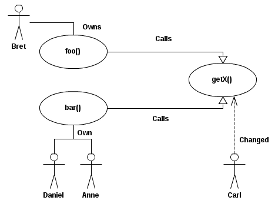
\includegraphics[width=0.5\textwidth]{images/CallGraph}
\caption{A method call graph with ownership.\label{fig:network}}
\end{figure}

\subsection{Information Visualization}



\section{Evaluation}

\subsection{Participants}

\subsubsection{Evaluation Strategy}



\section{Results}



\section{Discussion and Future Work}



\section{Threats to Validity}



\section{Conclusion}



\section{Acknowledgements}



\bibliographystyle{IEEEtran}
\bibliography{paper}

%End of paper
\end{document}